\documentclass[red]{beamer}
\usetheme{CambridgeUS}
\setbeamertemplate{navigation symbols}{}
\setbeamertemplate{footline}{}
\setbeamertemplate{items}[triangle] 
\renewcommand{\footnoterule}{}

\usepackage[utf8]{inputenc}
\usepackage[slovak]{babel}
\usepackage[IL2]{fontenc}
\usepackage[protrusion=true,expansion=true]{microtype}
\usepackage[none]{hyphenat}

\usepackage{hyperref}
\urlstyle{same}
\usepackage{textcomp}
\usepackage{xargs}
\usepackage{graphicx}
\usepackage{wrapfig}
\usepackage[absolute,overlay]{textpos}
\usepackage{amssymb}
\usepackage{amsmath}
\usepackage{verbatim}
\usepackage{eurosym}

\newcommand{\TODO}{{\color{red}!!!!!!!!!!!!!!!!!!!!!!!!}}
\newcommand{\vlnovka}{\raise.35ex\hbox{$\scriptstyle\mathtt{\sim}$}}

\newcommandx{\nadpis}[3][1=1,2]{\uncover<#1-#2>{\textbf{#3}}}
\newcommandx{\odrazka}[3][1=1, 2]{\begin{itemize}\item<#1-#2> #3\end{itemize}}
\newcommandx{\ukazka}[2][1=1,2]{\uncover<#1-#2>{\hspace{1cm}\textit{...demonstration...}}}
\newcommandx{\nadpisOnly}[3][1=1,2]{\only<#1-#2>{\textbf{#3}}}
\newcommandx{\odrazkaOnly}[3][1=1, 2]{\only<#1-#2>{\begin{itemize}\item #3\end{itemize}}}
\newcommandx{\ukazkaOnly}[2][1=1,2]{\only<#1-#2>{\hspace{1cm}\textit{...demonstration...}}}

\begin{document}

\large

\title{Počítačové videnie}
\subtitle{Rekonštrukcia Rubikovej kocky}
\author{Michal Bubnár, Michal Hozza, Matej Kopernický}
\date{13.12.2012}

{
\setbeamertemplate{background canvas}{
\includegraphics[width=\paperwidth,height=\paperheight]{title}}
\begin{frame}[plain,t]
\begin{center}
\color{white}
\vspace{2.3cm}
\huge\inserttitle\\
\vspace{1.2cm}
\Large\insertsubtitle\\
\vspace{1.5cm}
\color{black}
\large\insertauthor\\
\bigskip
\url{https://github.com/mhozza/rubik}
\end{center}
\end{frame}
}



\begin{frame}{Zadanie}
\odrazka[1]{Zrekonštruovať Rubikovu kocku z fotografie}
\medskip
\odrazka[2]{Získať 3D model kocky s farbami každého políčka na každej stene kocky}
\medskip
\uncover<1->{\centerline{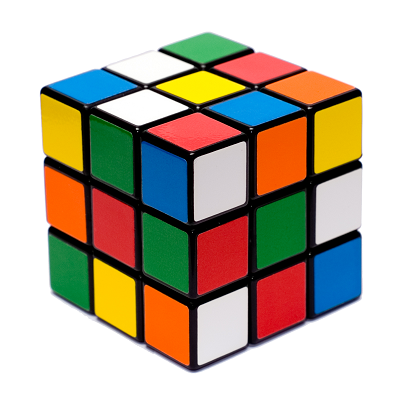
\includegraphics[width=.5\linewidth]{img/cube}}}
\end{frame}



\begin{frame}{Postup práce}
\odrazka[1]{Identifikovať pozíciu kocky na obrázku}
\pause
\odrazka[2]{Identifikovať pozíciu políčok na kocke}
\pause
\odrazka{Priradiť políčka k stene kocky a správne ich zoradiť}
\pause
\odrazka{Nájsť farbu každého políčka}
\pause
\odrazka{Vizualizovať výsledok}
%\centerline{\includegraphics[width=.8\linewidth]{depth_map_photo}}
\end{frame}



\begin{frame}{Postup práce}
\centerline{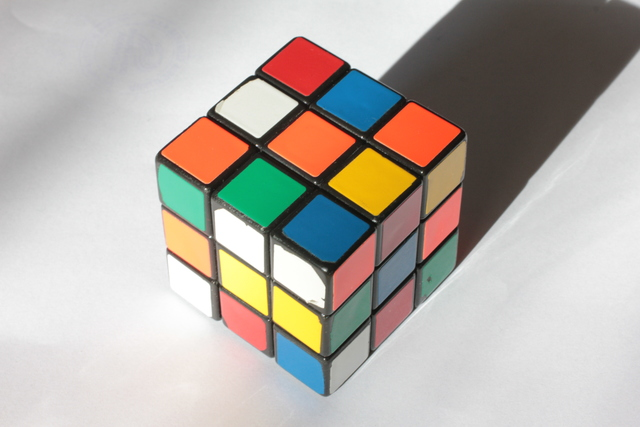
\includegraphics[width=.8\linewidth]{../images/IMG_2052.JPG}}
\end{frame}



\begin{frame}{Identifikácia kocky}
\odrazka{Hľadáme význačné charakteristiky kocky}
\bigskip
\pause
\odrazka{Prvý pokus -- nájsť čiary medzi políčkami pomocu Houghovej transformácie}
\pause
\odrazka{Bez úspechu}
\pause
\bigskip
\odrazka{Hľadanie políčok}
\pause
\odrazka{Nájdeme uzavreté oblasti na binárnom obrázku}
\end{frame}



\begin{frame}{Hľadanie hrán}
\odrazka{$E =$ zjednotenie hrán zo všetkých farebných zložiek + erózia}
\end{frame}



\begin{frame}{Hľadanie hrán}
\centerline{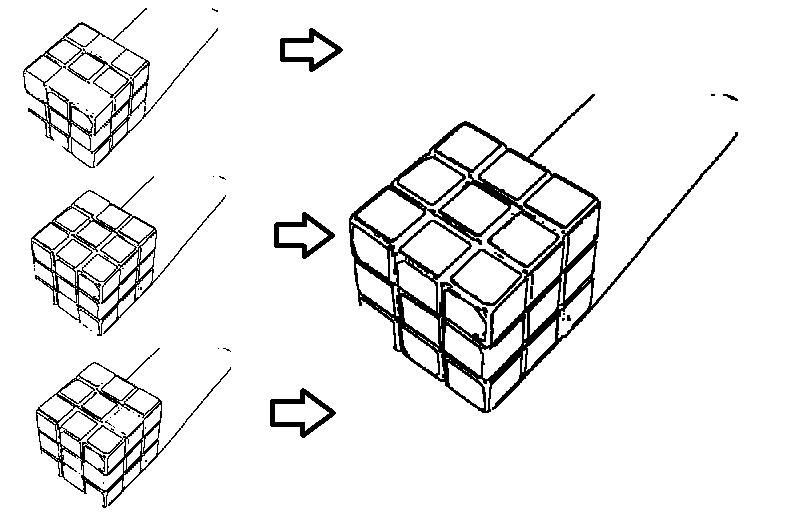
\includegraphics[width=.8\linewidth]{img/hranyRGBall}}
\end{frame}



\begin{frame}{Hľadanie hrán}
\odrazka{$E =$ zjednotenie hrán zo všetkých farebných zložiek + erózia}
\odrazka{$C =$ prienik jednotlivých farebných zložiek + erózia}
\end{frame}



\begin{frame}{Hľadanie hrán}
\centerline{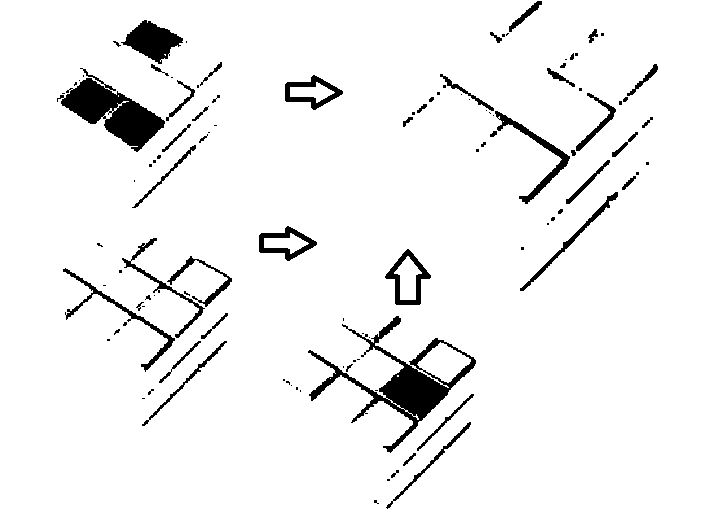
\includegraphics[width=.8\linewidth]{img/zlozkyRGBall}}
\end{frame}



\begin{frame}{Hľadanie hrán}
\odrazka{$E =$ zjednotenie hrán zo všetkých farebných zložiek + erózia}
\odrazka{$C =$ prienik jednotlivých farebných zložiek + erózia}
\odrazka{$C \cup E$ + erózia $=$ výsledný hranový obrázok}
\end{frame}



\begin{frame}{Hľadanie hrán}
\centerline{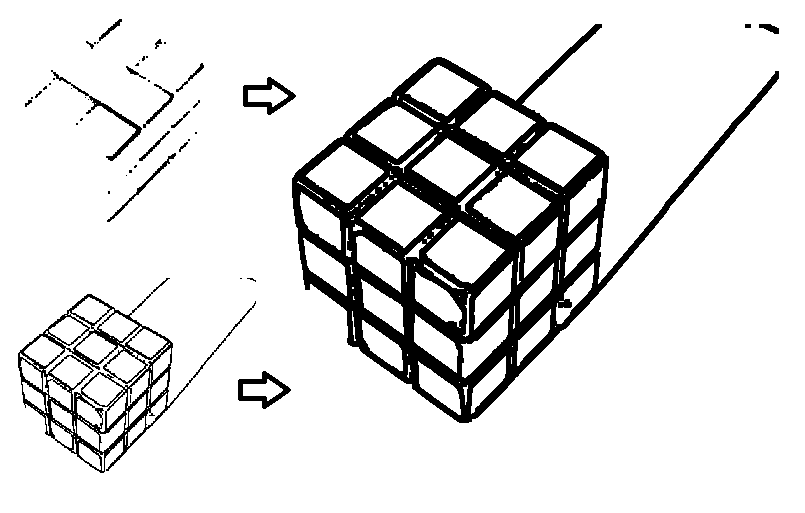
\includegraphics[width=.8\linewidth]{img/BWall}}
\end{frame}



\begin{frame}{Hľadanie políčok}
\odrazka{Chceme vyseparovať uzavreté oblasti}
\pause
\begin{itemize}
\item Použité množstvo kritérií
\begin{enumerate}[-]
\pause
\item Veľkosť oblasti
\pause
\item Pozícia oblasti na obrázku
\pause
\item Solidita oblasti
\pause
\item Pomer hlavnej a vedľajšej osi opísanej elipsy
\pause
\item Eulerovo číslo oblasti
\end{enumerate}
\end{itemize}

\pause
\begin{itemize}
\item Vylúčenie outlierov
\begin{enumerate}[-]
\pause
\item Vzdialenosť od najväčšieho zhluku
\pause
\item Vzájomné porovnanie veľkosti oblastí
\end{enumerate}
\end{itemize}
\end{frame}



\begin{frame}{Hľadanie políčok}
\centerline{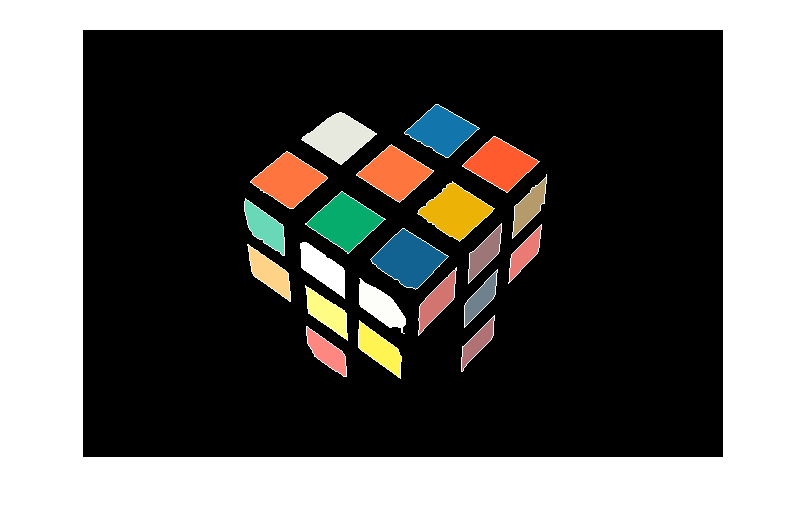
\includegraphics[width=\linewidth]{img/labels}}
\end{frame}



\begin{frame}{Zaradenie políčok}
\odrazka{Políčka chceme priradiť ku stene kocky a zoradiť ich v rámci steny}
\pause
\begin{itemize}
\item Nájdeme rohy políčok (ľavý horný/dolný, pravý horný/dolný)
\begin{enumerate}[-]
\pause
\item Line sweeping metóda s čiarami pod 45\textdegree uhlom
\pause
\item Optimalizázia počítaním skóre pre každý pixel obvodu
\end{enumerate}
\end{itemize}
\end{frame}


\begin{frame}{Zaradenie políčok}
\centerline{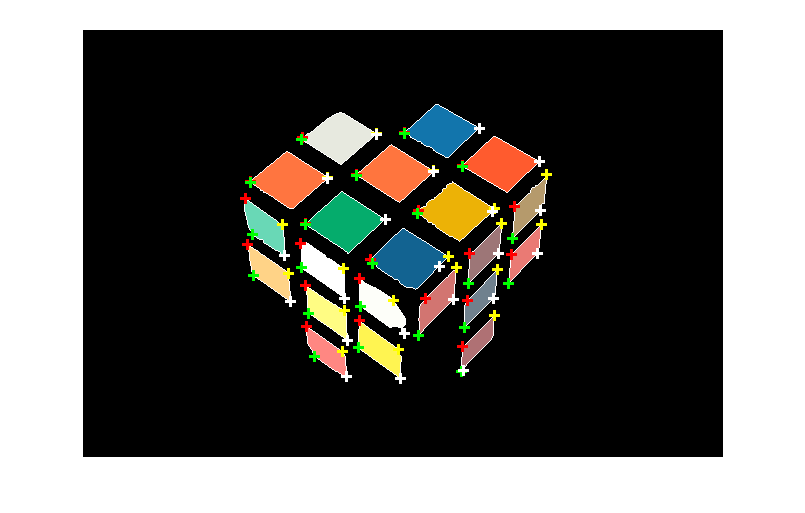
\includegraphics[width=\linewidth]{img/rohy}}
\end{frame}



\begin{frame}{Zaradenie políčok}
\odrazka{Políčka chceme priradiť ku stene kocky a zoradiť ich v rámci steny}
\begin{itemize}
\item Nájdeme rohy políčok (ľavý horný/dolný, pravý horný/dolný)
\begin{enumerate}[-]
\item Line sweeping metóda s čiarami pod 45\textdegree uhlom
\item Optimalizázia počítaním skóre pre každý pixel obvodu
\end{enumerate}
\end{itemize}
\odrazka{Zo vzájomnej pozície rohov vieme získať sklony hrán políčok}
\pause
\odrazka{Kritérium pre priradenie k stene kocky}
\pause
\odrazka{Eliminácia zle zaradených políčok na základe vzájomnej polohy}
\end{frame}



\begin{frame}{Zaradenie políčok}
\centerline{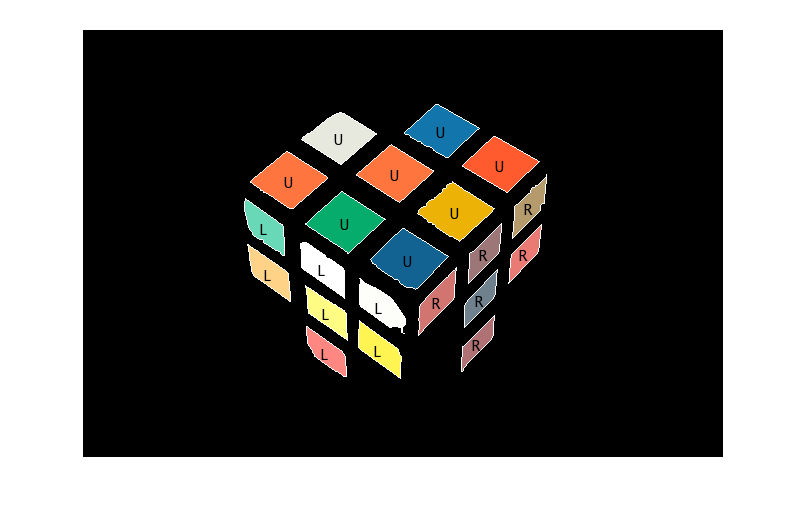
\includegraphics[width=\linewidth]{img/strany}}
\end{frame}



\begin{frame}{Chýbajúce políčka}
\odrazka{Nájdeme osi bočných strán kocky z hrán políčok}
\end{frame}



\begin{frame}{Chýbajúce políčka}
\centerline{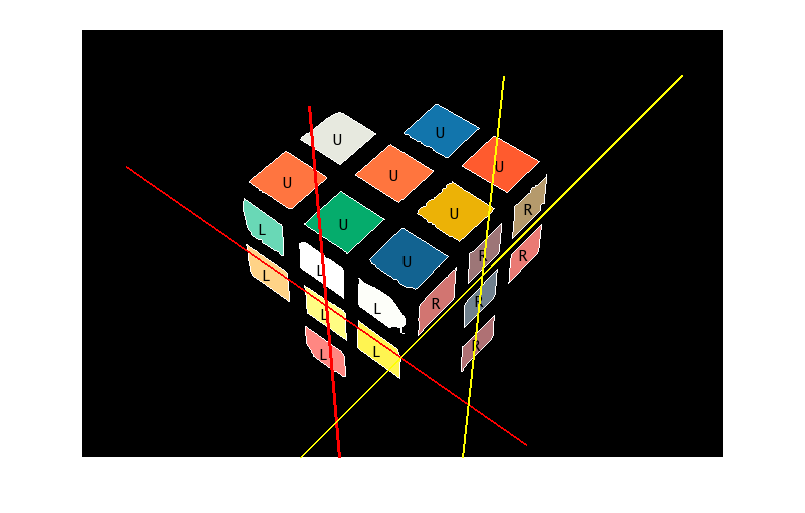
\includegraphics[width=\linewidth]{img/osi}}
\end{frame}



\begin{frame}{Chýbajúce políčka}
\odrazka{Nájdeme osi bočných strán kocky z hrán políčok}
\odrazka{Cez centroidy políčok vedieme osi a získame mriežku}
\pause
\odrazka{Pre hornú stenu použijeme osi bočných s kompenzáciou perspektívy}
\end{frame}



\begin{frame}{Chýbajúce políčka}
\centerline{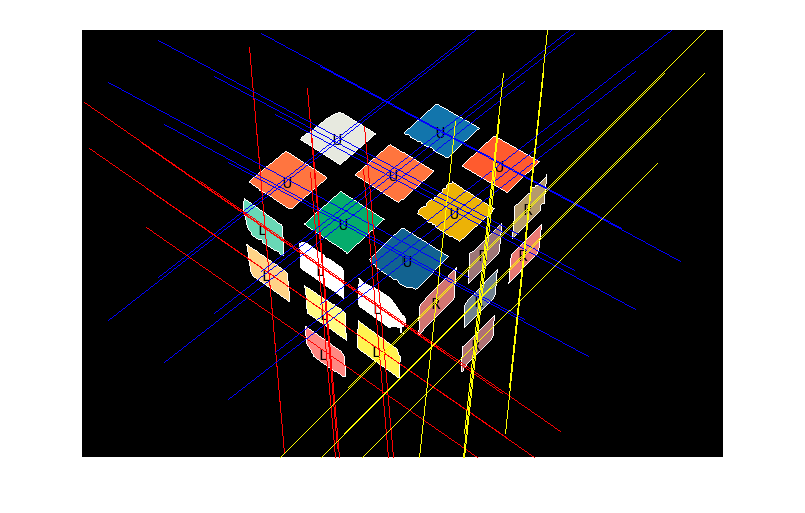
\includegraphics[width=\linewidth]{img/mriezka}}
\end{frame}



\begin{frame}{Chýbajúce políčka}
\odrazka{Priesečníky vedených osí sa stretnú v centroidoch políčok}
\pause
\odrazka{Priesečníky príliš vzdialené od známych políčok predstavujú chýbajúce}
\pause
\odrazka{Nájdeme zhluky pomocou k-means}
\end{frame}



\begin{frame}{Chýbajúce políčka}
\centerline{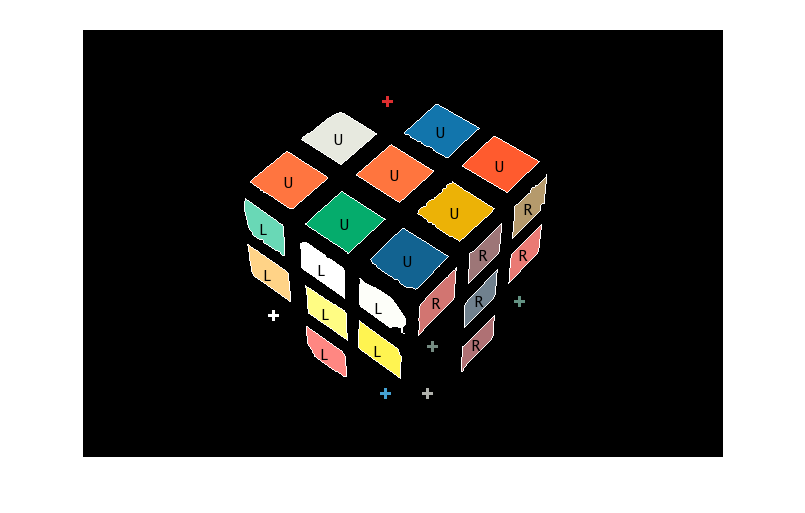
\includegraphics[width=\linewidth]{img/chybajuce}}
\end{frame}



\begin{frame}{Zoradenie políčok}
\odrazka{Pre vizualizáciu potrebujeme poznať aj poradie políčok v rámci steny}
\pause
\odrazka{Line sweeping pod uhlom osí pre získanie stĺpcov}
\pause
\odrazka{Políčka v stĺpci zoradíme podľa súradníc}
\end{frame}



\begin{frame}{Zoradenie políčok}
\centerline{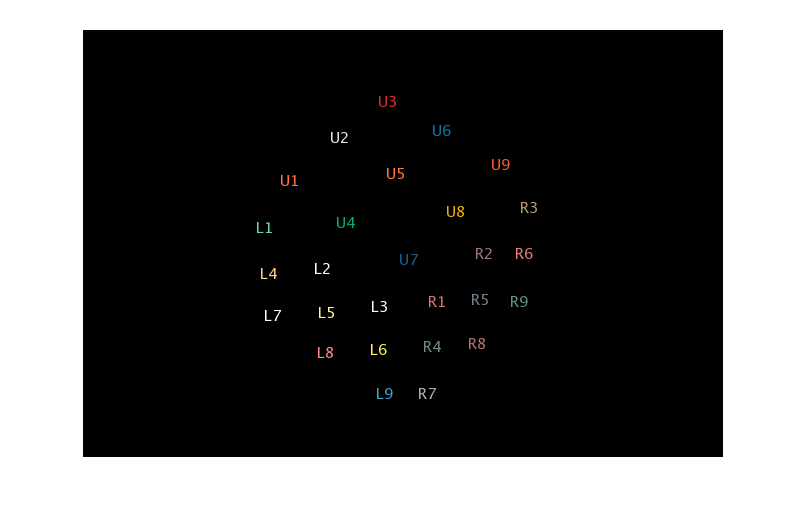
\includegraphics[width=\linewidth]{img/zoradene}}
\end{frame}



%%%%%%%% Matchovanie farieb %%%%%%%%%%
\begin{frame}{Priradenie nájdených farieb k farbám Rubikovej kocky}
\begin{textblock*}{3cm}(8.5cm,3.5cm)
\uncover<2->{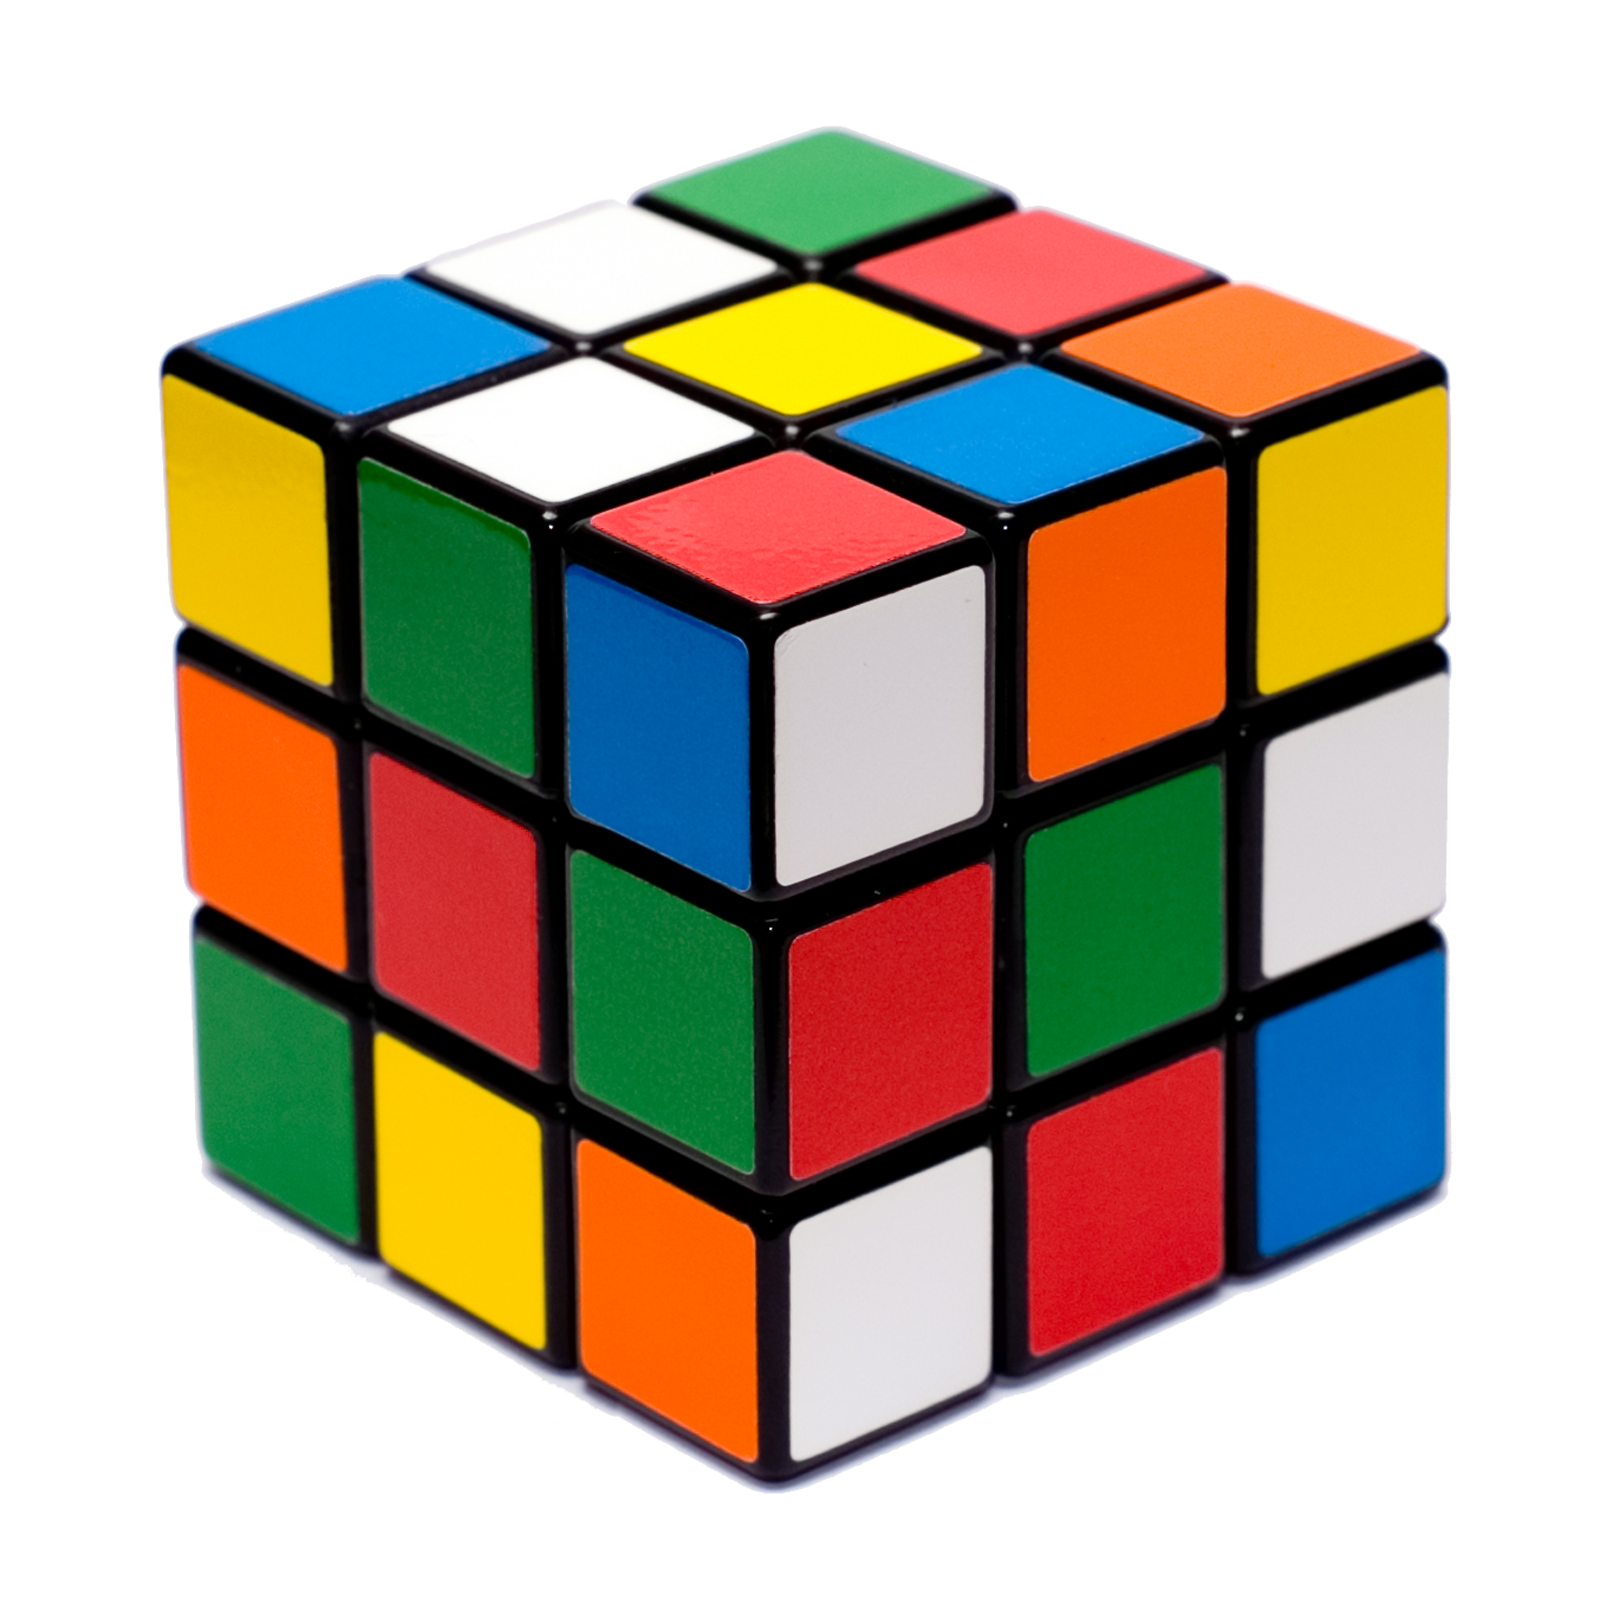
\includegraphics[width=\linewidth]{img/rubik}}
\end{textblock*}
\odrazka[1]{Chceme nájdené farby priradiť k farbám originálnej Rubikovej kocky}
\begin{itemize}
\item<2->{Rubikova kocka má 6 základných farieb}
    \begin{itemize}
    \item<2-> Red: $(196, 30, 58)$
    \item<2-> Green: $(0, 158, 96)$
    \item<2-> Blue: $(0, 81, 186)$
    \item<2-> Orange: $(255, 88, 0)$
    \item<2-> Yellow: $(255, 213, 0)$
    \item<2-> White: $(255, 255, 255)$
    \end{itemize}
\end{itemize}
\odrazka[3] {Jednoduchý algoritmus matchovania farby k farbe}
\odrazka[4] {Zložitejší algoritmus zgrupovania a matchovania skupiny k farbe}
\end{frame}



%%%%%%%% Matchovanie farby na farbu %%%%%%%%%%
\begin{frame}{Matchovanie jednej farby na farbu Rubikovej kocky}
\begin{itemize}
\begin{textblock*}{4.5cm}(8.0cm,5.5cm)
\uncover<2->{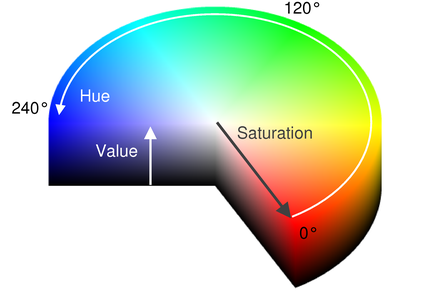
\includegraphics[width=\linewidth]{img/hsv}}
\end{textblock*}
%\item<1->Funkcia {\tt match\_color}:
\item<1->Prevod oboch farieb do HSV
\item<2->Spočítanie skóre pre všetky farby a následný výber farby s najväčším skóre
    \begin{itemize}
    \item<3-> rozdiel 2 farieb po zložkách   
    \item<4-> výsledné skóre je váhovaný súčet zložiek
    \item<5-> pre každú cieľovú farbu sú rôzne váhy
    \end{itemize}
\end{itemize}
\end{frame}

%%%%%%%% Zgrupovanie podobných farieb %%%%%%%%%%
\begin{frame}{Zgrupovanie podobných farieb}
\begin{itemize}

\begin{textblock*}{2.3cm}(9.3cm,3.6cm)
\uncover<2->{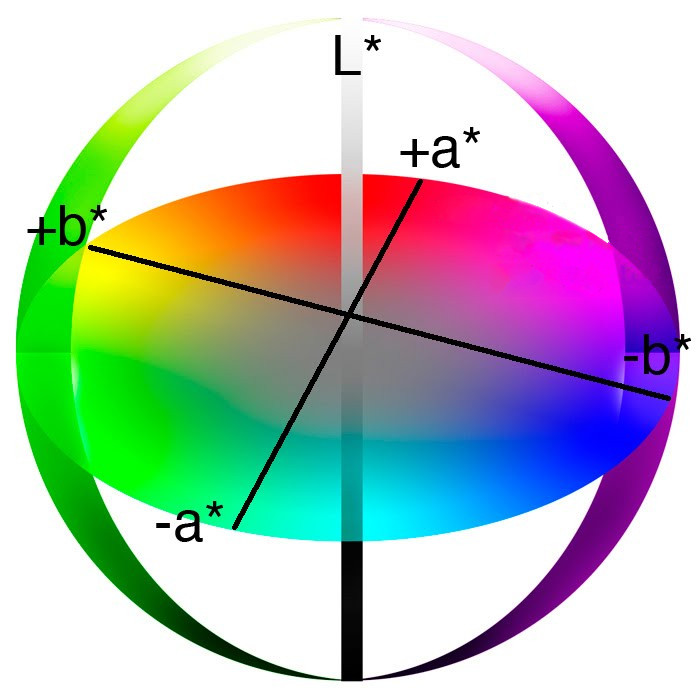
\includegraphics[width=\linewidth]{img/lab}}
\end{textblock*}

\item<1->Zgrupenie farieb podľa podobnosti, pre každú stranu zvlášť
    \begin{itemize}
    \item<2-> prevod do $Lab$
    \item<3-> euklidovská vzdialenosť na zložkách $a$, $b$\\
    $ d = \sqrt{(a_1-a_2)^2+(b_1-b_2)^2} $
    \item<4-> treshold na vyhodnotenie podobnosti
    \end{itemize}
\bigskip
\item<5-> Priradenie farieb ku grupám - nájsť čo najlepšie ohodnotenie farieb tak, aby žiadne 2 grupy nemali tú istú farbu
\end{itemize}
\end{frame}




\newcommand{\bibnet}[3]{#1: \textit{#2} [online]. \scriptsize$<$\mbox{\url{#3}}$>$\normalsize.}
\newcommand{\bibnetEllipsis}[4]{#1: \textit{#2} [online]. \scriptsize$<$\href{#3}{#4}$>$\normalsize.}

\begin{frame}{Literatúra}
\bibliographystyle{abbrv}
\begin{raggedright}
\begin{thebibliography}{9}
\bibitem{b1}
  \bibnetEllipsis{Justin Ng}{Automated Rubik's Cube Recognition}
  {http://www.stanford.edu/class/ee368/Project_12/Reports/Ng_Rubiks\%20Cube_Reconstruction_from_Images.pdf}
  {http://www.stanford.edu/class/ee368/Project\_12/Reports/...}
\bibitem{b2}
  \bibnet{Andrej Karpathy}{Extracting sticker colors on Rubik’s Cube}
  {http://karpathy.ca/portfolio/project525.php}
\bibitem{b3}
  W\l odzimierz Kasprzak, Wojciech Szynkiewicz, \L ukasz Czajka: \textit{Rubik's cube reconstruction from single view for Service robots}, Machine Graphics \& Vision International Journal archive, Volume 15 Issue 3, February 2006, Pages 451-459
\bibitem{b2}
  \bibnet{Yoann Bourse}{Controle 3D par un Rubik's Cube}{http://www.yoannbourse.com/ressources/docs/ens/stereovision.pdf}
\end{thebibliography}
\end{raggedright}
\end{frame}







\end{document}